\section{Visibility graphs}\label{sec:VisibilityGt}
	%\subsection{Historical roots}
	
	Another approach for transforming time series into complex network representations, which has recently attracted great interest, is the visibility graph (VG) algorithm. Originally, this concept has been introduced for the analysis of mutual visibility relationships between points and obstacles in two-dimensional landscapes in the framework of computational geometry, with applications ranging from robot motion planning to architectural design and topographic descriptions of geographical space \cite{Lozano1979,Nagy1994,Floriani1994,Turner2001}. Lacasa \emph{et al.}\cite{Lacasa2008} adopted the VG approach to the analysis of structures in scalar, univariate time series. Since this seminal work, different algorithmic variants of the original VG algorithm have been proposed, which we will summarize in course of this section. In general, visbility algorithms constitute a family of geometric and ordering criteria for scalar real-valued time series, providing a combinatorial representation of the underlying dynamical system \cite{Lacasa2018}.
	
	Some mini-review of VGs has already been presented in \cite{Nunez2012,Luque2016}. In particular, the application of this approach to geophysical time series has been focused on in \cite{Donner2012}, which has attempted to link the complete variety of different network properties describing the structure of VGs with specific structural features of geophysical processes in some more detail. Here, we summarize the recent developments of the method and discuss some practical issues which pose considerable challenges to VG analysis for experimental time series, such as missing data, homo- and heteroscedastic uncertainty of observations, and time-scale uncertainty. These practical problems for VG analysis have not yet fully answered since the early work of \cite{Donner2012}. In addition, we also discuss some successful applications of VGs and related methods to testing time-irreversibility of nonlinear time series. 
	
	\subsection{Algorithmic variants of visibility algorithms}
	In VG analysis, individual observations are considered as vertices. For instance, given a univariate time series $\{x_i \}_{i=1}^{N}$ with $x_i = x(t_i)$, the binary adjacency matrix $\mathbf{A}$ has size ${N \times N}$. Depending on the particular visibility conditions in defining the edges of the resulting graph, we can distinguish different versions of VGs. 
	
		\subsubsection{Natural visibility graphs}
		First, in the framework of the standard visibility graph (VG), the non-zero entries of $\mathbf{A}$ correspond to two time points $t_i$ and $t_j$ which are mutually connected vertices if the criterion 
\begin{equation} \label{vis_cond}
	\frac{x_i-x_k}{t_k - t_i} > \frac{x_i - x_j}{t_j - t_i}
\end{equation}
is fulfilled for all time points $t_k$ with $t_i < t_k < t_j$~\cite{Lacasa2008}. Therefore, the edges of the network take into account the temporal information explicitly. In Fig.~\ref{fig_chap04:timeseriesSS}(a), we illustrate the algorithm of constructing natural VGs for an example of a the sunspot time series. More detailed information on recent results obtained by VGs analysis of the sunspot series will be provides in Section~\ref{sec:appVGs}. 

By default, two consecutive observations are always connected in a VG, so that the graph forms a completely connected component without disjoint subgraphs. However, unlike for other types of time series networks, there are potentially relevant boundary effects, for instance, the first time point can only be visible to points that are in the future of this observation (Fig.~\ref{fig_chap04:timeseriesSS}(a)), see below for a detailed discussion. In turn, as an advantage, the VG is not affected by the choice of any algorithmic parameters -- in contrast to most other methods of constructing complex networks from time series data which depend on the choice of some parameters (e.g., the threshold $\varepsilon$ of recurrence networks, see more details in Section \ref{sec:RecurrenceNt}). 
		\begin{figure}
		  \centering
		  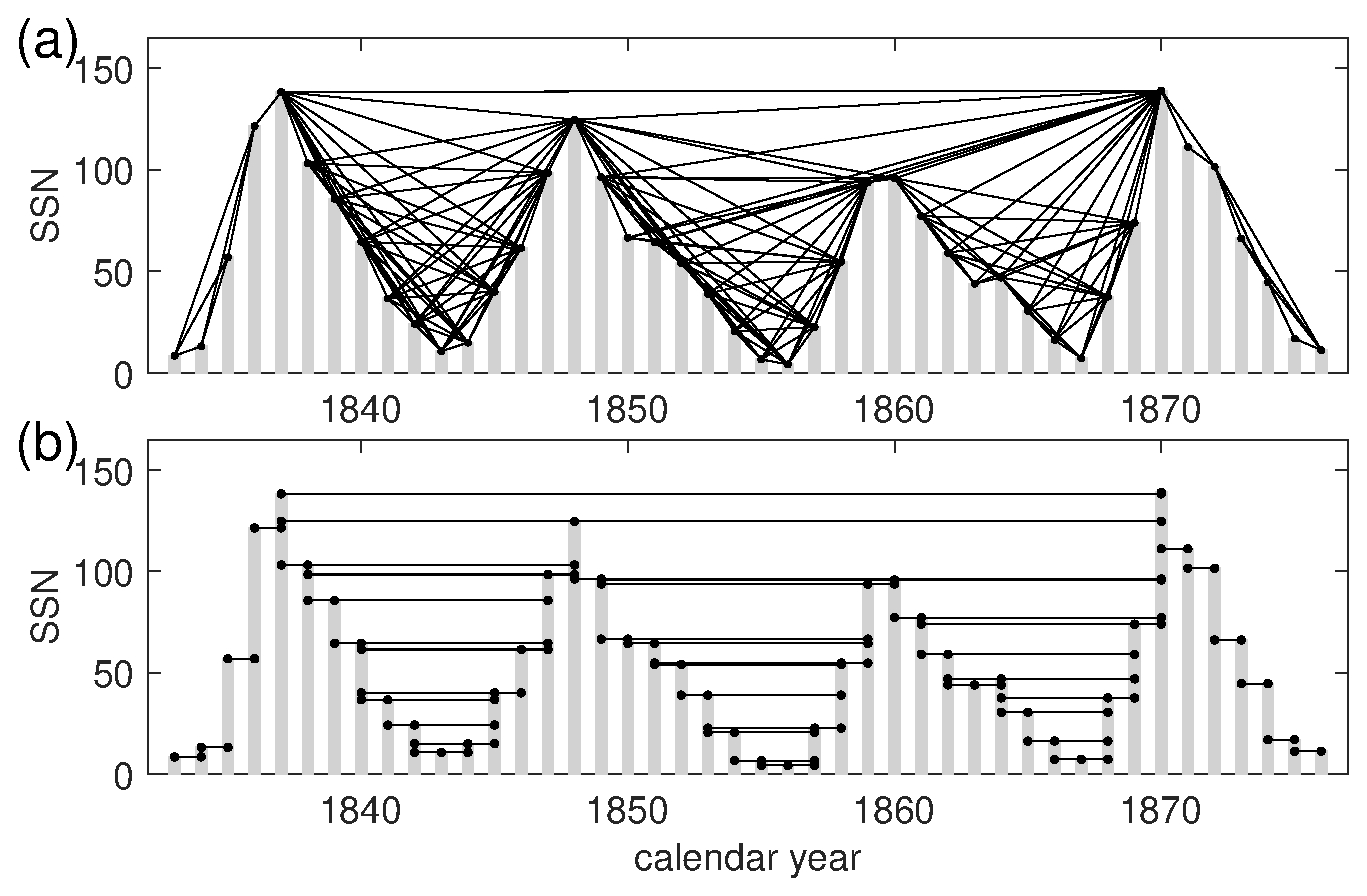
\includegraphics[width=0.8\columnwidth]{Chapter04_VisibilityGt/TSspotnumberYear.eps}
		  \caption{Schematic illustration of the algorithm for constructing (a) natural visibility graphs and (b) horizontal VG for an excerpt of the time series of sunspot numbers. Reproduced from \cite{Zou2014}. \label{fig_chap04:timeseriesSS}}
		\end{figure}
		
		\subsubsection{Horizontal visibility graphs}
		As a notable modification of the standard VG algorithm, Luque \textit{et al.} \cite{Luque2009,Lacasa2010} proposed utilizing a simplified criterion of horizontal visibility for transforming a time series into a complex network. Specifically, they considered two observations made at times $t_i$ and $t_j$ to be connected in a horizontal visibility graph (HVG) if and only if
\begin{align}
x_k < \min \left\{ x_i, x_j \right\} \label{eq:hvc}
\end{align}
for all $t_k$ with $t_i<t_k<t_j$. 

		The algorithmic difference between HVG and VG is illustrated in Fig.~\ref{fig_chap04:timeseriesSS}(b). Note that the geometric criterion defining the HVG algorithm is more ``visibility restrictive" than its analogous for the standard VG. That is to say, the nodes within a HVG will have ``less visibility" than their counterparts within a VG. It is easily seen that the edge set of the HVG associated with a given time series is a subset of the edge set of the associated VG, which means that if the horizontal visibility criterion in Eq.~(\ref{eq:hvc}) is fulfilled, then also Eq.~(\ref{vis_cond}) holds, but not necessarily vice versa. In addition, VGs are invariant under affine transformations of the entire time series, whereas HVGs are not. One notable advantage of HVGs is that they provide an even higher degree of algorithmic simplicity than standard VGs, resulting in the observation that for certain simple stochastic processes and the quasiperiodic transition route to chaos, some basic graph properties can be calculated analytically \citep{Luque2009,Luque2013a,Luque2013d}. On the other hand, the fact that HVGs typically contain a lower number of edges increases the demands regarding the time series length relative to those of the standard VG when using this approach in applications, such as tests for time-reversal asymmetry \citep{Donges2013} (see Section~\ref{sec:timeIRvg}). 
		
        To further account for the differences between natural and horizontal visibility graphs, Zhu \textit{et al.} \cite{Zhu2014b} introduded the concept of \emph{difference visibility graphs (DVGs)}, which are based on the node and edge sets of the natural VG with the edges of the HVG being removed, i.e., $E_{DVG}=E_{VG}\backslash E_{HVG}$ and $V_{DVG}=V_{VG}=V_{HVG}$. This construction immediately implies that the degree sequence of the DVG is defined as the (strictly non-negative) difference series between the degree sequences of the VG and HVG, respectively. Wang \textit{et~al.} \cite{Wang2017} recently demonstrated that the degree properties of DVGs obtained from EEG data can be employed to differentiate between different types of epileptic seizures.
        
		\subsubsection{Other variants of (H)VG}
		Throughout this section, we will mostly focus on the discussion of the standard VG and horizontal VG algorithms and their applications. However, there are some other generalizations of these two algorithms that will be briefly summarized in the following. Recent applications of the (H)VG algorithms and their variants to experimental time series of various origins will be reviewed in Section \ref{sec:appVGs}. 
		
		Given the definitions of VG and HVG, the resulting graphs are undirected and unweighted. One straightforward generalization of (H)VGs to \emph{directional (H)VGs} is to introduce directed edges between vertices, i.e., from the cause at $t_i$ to the effect at $t_j > t_i$. As it will be shown in Section~\ref{sec:timeIRvg}, such directed graphs provide information on time-reversal asymmetry of the considered time series. 
        
        Since an edge represents the visibility between two time points $t_i$ and $t_j$ that can be either consecutive in time or be separated by various other observations, another generalization of the original ideas of (H)VGs is to construct a \emph{weighted (H)VG} which takes into account the time distance between $t_i$ and $t_j$ \cite{Bianchi2017}. More specifically, the weight $w_{ij}$ is defined as $w_{ij} = 1 / \sqrt{(t_j - t_i)^2 + (x_j - x_i)^2} \in [0, 1]$. Thereby, these weights capture time distance information $(t_j - t_i)$ as well as amplitude differences $(x_j-x_i)$ of two data points connected by the respective visibility rule. The corresponding approach has been applied to characterize heterogeneity of recurrent neural network dynamics \cite{Bianchi2017}. 
		
		There are several further algorithmic variants of (H)VG that address specific properties of time series. For instance, given a binary series, in \cite{Ahadpour2012}, a simplified VG has been developed yielding a \emph{binary VG}, in which the visibility condition (Eq.~\ref{vis_cond}) is reduced to $x_i + x_j > x_k$ for all $t_k$ such that $t_i < t_k < t_j$. The resulting VG from binary series is always connected and undirected and more easily tractable than the standard VGs. 
		
		\emph{Parametric VGs} have been proposed in \cite{Bezsudnov2014,Snarskii2013a}, introducing ``viewing angle'' $\alpha$. When this angle $\alpha = \pi$, the parametric VG and the standard VG are the same. However, the angle $\alpha = \pi / 2$ does not turn into HVG because $\alpha$ introduces a direction of links in the resulting graph. By means of this algorithm, it is possible to study the dependence of network structural measures on the parameter $\alpha$. 
		
		The concept of \emph{limited penetrable VG} (LPVG) \cite{Zhou2012,Gao2013e} can be regarded as a continuous construction of a HVG based on a properly coarse-grained time series. In the original HVG, two time points $t_i$ and $t_j$ are connected if no other intermediate points $x_k$ are larger than $\min{x_i, x_j}$. Now we use a less restrictive criterion, allowing one of $x_k$ to be larger than $\min{x_i, x(_j}$, as represented by the new parameter of $L=1$. Similarly, we allow two points $x_k$ larger than $\min{x_i, x_j}$ if $L = 2$, etc. When increasing $L$, there are more edges in the resulting LPHVGs as compared to the standard HVG. The standard VG is recovered from the LPVG if $L \to \infty$. A straightforward extension in terms of the multi-scale \emph{limited penetrable HVG algorithm} (LPHVG) has been proposed in \cite{Gao2016,Pei2014a} and successfully applied to the analysis of EEG time series \cite{Wang2016} and electromechanical signals \cite{Wang2016b}. Recently, the limited penetrable VG algorithm has been combined with a parametric VG in \cite{Li2018}. Moreover, the key topological characteristics of LP(H)VGs have been studied in great detail in a series of papers \cite{Wang2018,Wang2018b,Wang2018c}.
				
		An extension of (H)VGs from a univariate time series to scalar fields has been recently reported in \cite{Xiao2014a,Lacasa2017}, which is conceptually closer to the original idea of visibility graphs. In addition, one may reconstruct (H)VGs for a set of ordered data (either in descending or increasing order) \cite{Wang2015a}. 
						
		It is also possible to combine the concepts of VGs with transition networks (Section~\ref{sec:TransitionNt}), e.g., by using the \emph{visibility graphlet} approach proposed in \cite{Mutua2015,Mutua2016a}. In this case, VGs are constructed for sliding windows, and each window is regarded as a network node. The connection between two nodes represents their temporal succession. The resulting transition network is regular for periodic dynamics while showing more complex structural properties for chaotic systems \cite{Mutua2016a}. The computation of network measures (including the average path length and network diameter) have successfully tracked the different bifurcations from period doubling and intermittency to chaos in the logistic map. 
		
		In all above cases, (H)VGs have been constructed from a given time series. In \cite{Tsiotas2018}, Tsiotas {\textit {et al.}} expanded the VG algorithm to analyze node attributes of a given graph. More specifically, let us consider a graph $G(V, E)$ and a node attribute $Y$ that might be any of the node-wise network measures, e.g., local clustering coefficient or betweenness centrality. The secondary VG analysis for node-wise attributes $Y$ shows a specific capability in pattern recognition \cite{Tsiotas2018}. 
				
		Other properties of combinatorics have been used to characterize HVGs successfully in \cite{Gutin2011}. Recently, some analytic results have been obtained for independent and identically distributed random noise, which has an exponential degree distribution \cite{Wang2018}. 

		The time complexity of the basic natural VG algorithm is $O(N^2)$, which means that it takes a lot of time when dealing with long time series. A faster transform algorithm has been proposed in \cite{Lan2015a} to reduce the computation time, showing much more efficient time complexity $\sim O(N \log N)$. Note that for the HVG algorithm, it is not possible to further improve the computational efficiency because it has already reached the lower bound $\sim O(N)$. 
		
	\subsection{Visibility graph properties}
		\subsubsection{Degree distributions}
		A vast body of early works on (H)VGs has mainly concentrated on the properties of the degree distribution $p(k)$ resulting from different kinds of processes. Specifically, VGs obtained from periodic signals appear as a concatenation of a finite number of network motifs (given that the basic period is an integer multiple of the sampling rate), i.e., have a regular structure with only a few distinct values of the vertex degree. The opposite extreme case, white noise, yields VGs appearing as exponential random graphs, i.e., random networks characterized by an exponential degree distribution. For example, exponential degree distribution have been reported for wind speed records measured in central Argentina \cite{Pierini2012}. 
		
		In fractal processes, numerical results suggest that $p(k)$ exhibits a power law \cite{Lacasa2008}, $p(k) \sim k^{-\gamma}$. Taking this empirical observation, VG analysis has been suggested to characterize fractional Brownian motions and $f^{\beta}$-noise, finding some heuristic relationship between $\gamma$ and the process Hurst exponent $H$ as $\gamma = 3 - 2H$, and $\gamma = 5 - 2H$ for fractional Gaussian noise \cite{Lacasa2009,Ni2009}. Depending on the fractal properties of the underlying process, recently a resampling algorithm for constructing VGs from segmented time series has been proposed \cite{Ahmadlou2012}, which estimates power-law exponents reflecting SF properties quite well. This improved algorithm has been applied to diagnose Autism spectrum disorders \cite{Ahmadlou2012}. Since there are many concerns regarding the statistical justification of the power laws of VGs, one can directly analyze the degree sequence (instead of the distribution) by detrended fluctuation analysis \cite{Czechowski2016}, which quantifies the multifractal properties better than standard VGs analysis.  
	
		Some exact results of $p(k)$ for HVGs associated with generic uncorrelated random series have been obtained in \cite{Luque2009}. More specifically, for a bi-infinite time series created from a random variable $X$ with the probability distribution $p(x)$ and $x\in [0, 1]$, it has been proven that the degree distribution of the graph has an exponential form 
		\begin{equation}\label{pkhvg}
		p(k) = \frac{1}{3} \left(\frac{2}{3}\right)^{k-2}. 
		\end{equation}
Interestingly, for every probability distribution $p(x)$ of uncorrelated random series, we find the same exponential form for the HVG's degree distribution. Numerical results for $p(x)$ with a uniform, Gaussian and power-law form (e.g., $p(x) \sim x^{-2}$) show perfect agreements with this theoretical prediction \cite{Luque2009}. A general diagrammatic theory has been proposed in \cite{Lacasa2014b} to compute $p(k)$ for any given dynamical process with well-defined invariant measure. Taking into account the time information explicitly as in so-called directed HVG (as will be explained below), the outgoing degree distribution $p_{out}(k) = (1/2)^{k}$. Further solvable examples include Markovian processes with an integrable invariant measure $p(x)$, for instance, the stationary Ornstein-Uhlenneck process, and one-dimensional chaotic and quasi-periodic maps of with smooth invariant measure. In addition, the mean degree $\left< k \right>$ of the HVG associated with an uncorrelated random process is then given by 
\begin{equation}
\left< k \right> = \sum k p(k) = \sum_{k=2}^{\infty} \frac{k}{3}\left(\frac{2}{3}\right)^{k-2} = 4.
\end{equation}
For an infinite periodic series of period $T$, the mean degree is $\left< k \right> = 4 ( 1 - \frac{1}{2T})$. 
	
		Similar to VGs, HVGs have been successfully applied to studying time series from various fields of sciences. We particularly notice a recent paper \cite{Yu2012} which studied the multifractal properties of some solar flare index in terms of HVG characteristics. Among others, the properties of HVGs have been studied in river flows \cite{Braga2016}, showing exponential degree distributions. 
		
		In order to understand the hypothetical SF property of $p(k)$ for VGs from fractal records, one has to note that typically, maxima of the time series have visibility contact with more other vertices than other points, i.e., hubs of the network often form at maximum values of the recorded observable. Put it differently, the degree of a vertex in the VG characterizes the maximality property of the corresponding observation in comparison with its neighborhood in the time series. Although locally large time series values have better visibility than other small values, hub nodes of large degrees of VGs do not necessarily correspond to higher values, especially when there is some sort of periodic trend in the given data sequence, for instance, in wind speed records \cite{Pierini2012,Zou2014a}. Therefore, the relationship between maxima time series points and hubs of VGs is not completely general, since there can be specific conditions (e.g., a concave behavior over a certain period of time) which can lead to highly connected vertices that do not coincide with local maxima, for example, in case of a Conway series \cite{Lacasa2008}. 
				
		In addition, studying the minima of a given time series provides complementary insights for the understanding of the particular process, for instance, in case of sunspot series \cite{Zou2014a}. In standard VGs, the contributions of local minimum values are largely overlooked by the degree distribution $p(k)$ because minimum values are basically represented by non-hubs. One simple solution is to study the negative counterpart of the original time series, $\{-x_i\}$, the VG of which highlights the properties of the local minima \cite{Zou2014a}. For convenience, we use $k^{-x}_i$ and $P(k^{-x})$ to denote the degree sequence and distribution of VG resulting from $\{-x_i\}$. Here, we remark that this simple inversion of the time series allows us to create an entirely different complex network. This technique has demonstrated to be useful to understand the long-term behavior of strong minima of solar activity \cite{Zou2014a}. We will review these results in Section~\ref{subsec:sunnum}. 
		
		The graph entropy is often computed as $\mathcal{S} = - \sum_{k} p(k) \log p(k)$ and is used as the approximation to the Shannon entropy $S$ of the corresponding time series $\{x_i\}$ \cite{Luque2016,Goncalves2016}. Furthermore, based on the degree sequences, the VG aggregation operator has been proposed in \cite{Chen2014,Jiang2016}. This operator includes temporal information in the weights of the aggregation, showing computational simplicity comparing to other traditional aggregation operators.  
					
		\subsubsection{Distinguishing stochastic and deterministic dynamics}
		For the HVG, exponential functional forms, $p(k) \sim e ^{-\lambda k}$, have been found for many random processes. A scaling factor of $\lambda_c = \ln (3/2)$ has been found in the case of uncorrelated noise (white noise), which has been further proposed to separate stochastic from chaotic dynamics in the following senses \cite{Lacasa2010,Lacasa2014b,Ravetti2014}: (i) correlated stochastic series are characterized by $\lambda > \lambda_c$, slowly tending to an asymptotic value of $\ln (3/2)$ for very weak correlations, whereas (ii) chaotic series are characterized by $\lambda_{chaos} < \lambda_c$ for decreasing correlations or increasing chaos dimensionality, respectively \cite{Lacasa2010}. In \cite{Zhang2017}, Zhang {\textit{et al.}} have provided some further examples supporting argument (i). Meanwhile, some peculiar results have been found indicating that $\lambda_c$ should not be interpreted as a general critical value separating chaos from noise \cite{Ravetti2014}. 
		
		Let us focus on applying (H)VG analysis to auto-regressive (AR) stochastic processes, which often describe a general model for colored noise as an idealization of time-varying processes in nature, economics, etc. The AR model specifies that the output variable depends linearly on its own previous values and on a stochastic term (Eq.~\ref{def:AR}). More specifically, we perform both VG and HVG analysis for stationary AR(1) processes, i.e., with $|\varphi_1| < 1$ where $\varphi_1$ is the characteristic parameter of the AR(1) model. It is known that $\varphi_1 > 0$ corresponds to positive correlations and the correlation length increases when $\varphi_1$ increases from 0 to 1. In contrast, anti-correlation is observed for negative coefficient $\varphi_1$. Similar H(VG) analysis for the AR(2) model has been reported in \cite{Zhang2017}. 

		In the case of $\varphi_1 > 0$, we find that $p(k)$ approximately follows an exponential distribution. To illustrate this finding, the complementary cumulative degree distributions $F(k)$ for $\varphi_1 = 0.3 $, $0.9$ and $-0.5$ are shown in Fig. \ref{fig:lambda_AR1}(a) and (b), where clear scaling regimes are present in the semi-logarithmic plots. Furthermore, when increasing $\varphi_1$, in the VG, the exponent $\lambda$ shows a monotonically decreasing trend (Fig.~\ref{fig:lambda_AR1}(c)). In contrast, the value $\lambda$ for the HVG is increased (Fig.~\ref{fig:lambda_AR1}(d)). The result of Fig.~\ref{fig:lambda_AR1}(d) confirms the hypothesis stated in \cite{Lacasa2010} that all $\lambda$ should be larger than $\lambda_c = \ln (3/2)$ as the correlation length is increased in the case of positively correlated increments.
\begin{figure}
	\centering
	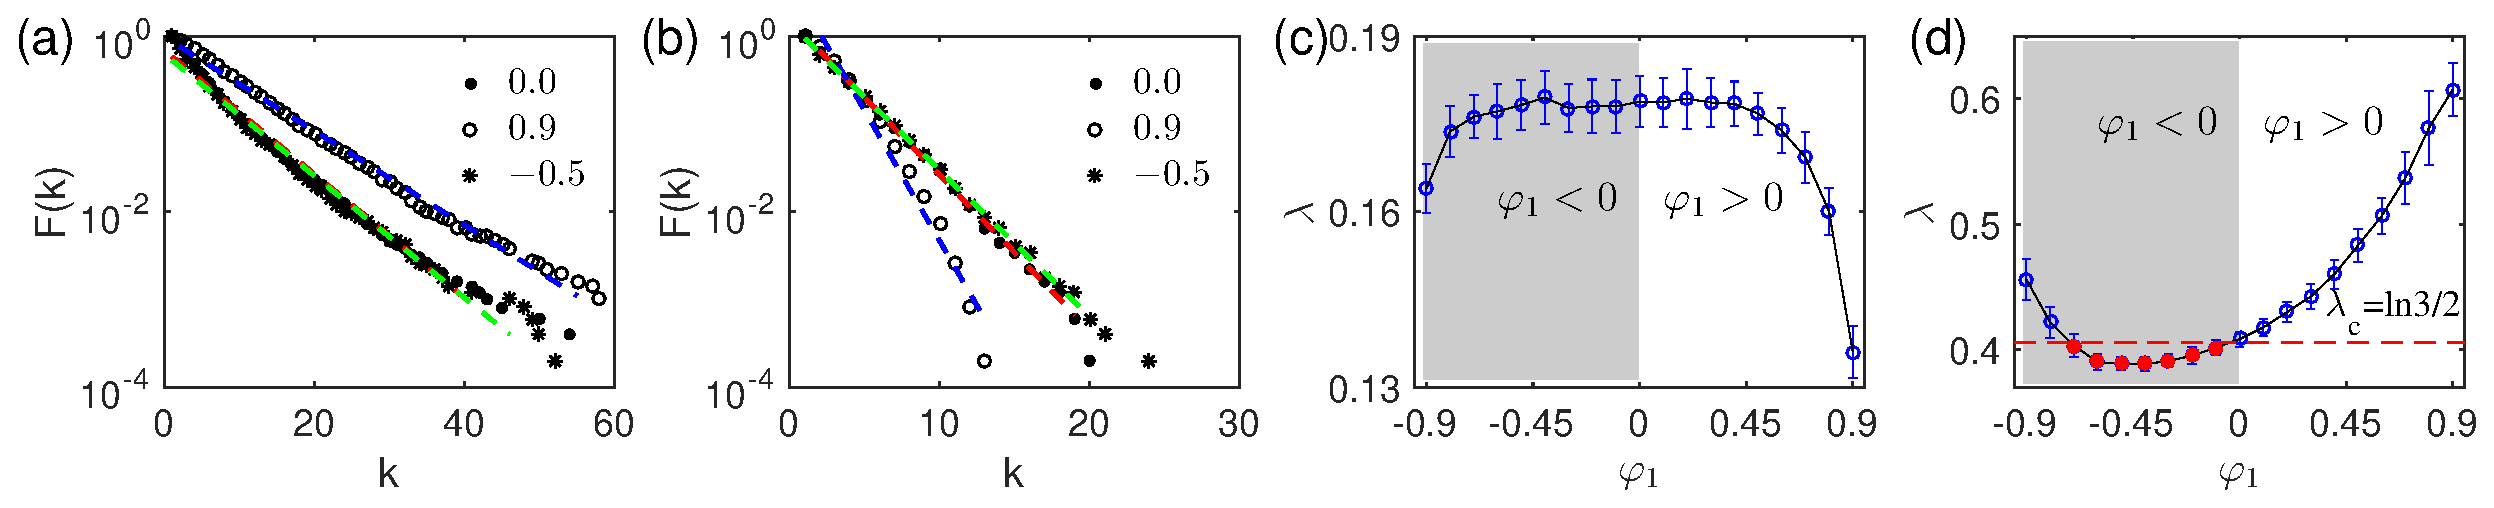
\includegraphics[width=\columnwidth]{Chapter04_VisibilityGt/ar1_positive_lambda_vg_hvg.eps}
\caption{(color online) (a, b) Estimates of $\lambda$ for approximately exponential degree distributions of the AR$(1)$ process. (c, d) $\lambda$ versus $\varphi_1$. (a, c) VG, and (b, d) HVG. Each dot in panels (c) and (d) represents an average over 50 independent random realizations of 5000 data points. In (d), $\lambda$ values smaller than $\ln 3/2$ are highlighted by red color. Reprinted from \cite{Zhang2017} with permission of the original publisher. \label{fig:lambda_AR1}}
\end{figure}

		In turn, when $\varphi_1 < 0$, we observe some peculiar results that seem to contradict the original hypothesis of \cite{Lacasa2010} that $\lambda$ should be larger than $\lambda_c$ ($\lambda > \lambda_c$) in stochastic processes. Notably, the results of Fig.~\ref{fig:lambda_AR1}(d) do not support this claim when $\varphi_1$ is negative in the AR(1) model. Instead, we find a region where the slope of the exponential degree distribution is smaller than $\ln (3/2)$ (as highlighted in Fig.~\ref{fig:lambda_AR1}(d)). This suggests that the critical value of $\ln (3/2)$ should not be understood as a general law for separating correlated stochastic from chaotic processes, which requires further investigation. 

		Working with correlated stochastic time series, further results in \cite{Manshour2015} do not adequately support the arguments of exponential degree distributions as reported in \cite{Lacasa2010}. More specifically, they have constructed (H)VGs for fractional time series with three different methods, a generic $1 = 1 / f^{\beta}$ noise constructed by Fourier filtering, a deterministic fBm process of the Weierstrass-Mandelbrot function, and a stochastic fBm process generated with a successive random addition method. Numerical analysis shows that the VG algorithm may not provide a good method to extract correlation information of a time series and its statistics is not essentially the same as that of the HVG. The degree distributions of HVGs are shown to have parabolic exponential forms with the fitting parameter depending on the Hurst exponent \cite{Manshour2015}. 
		
        \subsubsection{Degree sequences of horizontal visibility graphs}
        
        Due to their specific construction procedure, the degree sequences of HVGs carry essential information on the properties of the system under study. Notably, it can be shown that there exists a bijection between the degree sequence and the associated adjecency matrix of HVGs \cite{Luque2017b}. Even more, the degree sequence of a HVG can be interpreted as a symbolic discretization of the underlying time series (i.e., a transformation from real into integer-valued observations). By studying the scaling of the associated block entropies of degree subsequences, Lacasa and Just \cite{Lacasa2018} demonstrated the convergence of these block entropies towards the Kolmogorov-Sinai entropy of the system, indicating that the degree sequence asymptotically fulfills the properties of a generating partition of the system under study and, hence, provides an encoding without information loss.
        
        
		\subsubsection{Local network properties}
		\paragraph{Local clustering coefficient $\mathcal{C}_i$} 
		In the case of VGs, the local clustering coefficient $\mathcal{C}_i$ and its relationship with the degree $k_i$ have been numerically studied recently in human heartbeat data \cite{Shao2010}. Particularly, it has been observed that $\mathcal{C}(k) \sim k^{-\gamma}$ and $\gamma = 1$, pointing to a hierarchical organization of the network \cite{Albert2002}, since vertices $i$ with high $\mathcal{C}_i$ and low $k_i$ (which are most abundant) form densely connected subgraphs, indicating a strong modular structure of the VG. 

		In the case of HVGs associated an uncorrelated random series, $\mathcal{C}_i$ can be easily deduced by means of geometrical arguments. For a given vertex $i$, $\mathcal{C}_i$ denotes the fraction of nodes connected to $i$ that are connected between each other. In other words, we have to calculate from a given vertex $i$ how many vertices from those visible to $i$ have mutual visibility (triangles), normalized with the cardinality of the set of possible triangles, $\binom{k}{2}$, where $k$ is the degree of vertex $i$. Based on a general rule between the degree $k$ and the local clustering coefficient
		\begin{equation}
		\mathcal{C}_v(k) = \frac{k-1}{\binom{k}{2}} = \frac{2}{k}, 
		\end{equation}
one obtains the distribution $p(\mathcal{C})$ as 
		\begin{equation}
		p(\mathcal{C}) = \frac{1}{3} \left(\frac{2}{3}\right)^{2/\mathcal{C} -2}. 
		\end{equation}
The above theoretical result has been numerically confirmed for uncorrelated random series \cite{Luque2009}. In addition, for HVG of a binary sequence, $p(\mathcal{C})$ has a simplified expression as reported in \cite{Ahadpour2012}. 
			
		\paragraph{Betweenness $b_i$}
		In many cases local maxima of the underlying time series are expected to have large values of betweenness because high values often correspond to hubs in VGs which separate different parts of the series without mutual visibility contact and, thus, act as bottlenecks in the network structure, bundling a large number of shortest paths between vertices at $t < t_i$ and $t > t_i$, respectively. However, in contrast to $k_i$, $b_i$ is additionally affected by the vertex' position in the underlying time series due to a simple combinatorial effect: Considering that the majority of shortest paths that cross a vertex $i$ connecting observations before and after $i$ with each other, there are more possible combinations of such points for $i$ being close to the middle of the time series than for vertices close to the edges of the record. In this respect, in a VG betweenness centrality of a vertex mixes information on the local maximality of the corresponding observation and its position within the time series.
		
		\paragraph{Closeness centrality $c_i$}
		The position of a vertex in the time series is even more important for the closeness centrality $c_i$. Specifically, $c_i$ is strongly determined by the number of vertices to its left and right, respectively. In this spirit, it can be argued that in the middle of the time series, high values $c_i$ are more likely than at its ends. As argued above, a similar (but weaker) effect contributes to betweenness and - close to the edges of the record - also to the degree (consequently, the highest degree and betweenness values can be taken by other vertices than that corresponding to the global maximum). In contrast, $\mathcal{C}_i$ is almost unaffected except for vertices very close to the beginning and end of the time series, since direct connectivity is mainly established between vertices that correspond to observations that are not very distant in time. 
		
		From the above discussion, we note that boundary effects play an important role in the computation of the local centrality measures as that has been numerically reported in \cite{Donner2012}. Except for $\mathcal{C}_i$, the impact of boundaries on the estimated vertex properties is particularly strong for short records, which is typical for many observational time series. In particular, degree and other centrality properties of observations close to both ends of a time series are systematically underestimated, which may artificially alter the interpretation of the corresponding results in their specific context. Hence, a careful treatment and interpretation of the results of VG analysis is necessary in such cases \cite{Donner2012}.
				
		\subsubsection{Global network properties}
		The edge density $\rho$ of a (H)VG is a true network characteristic rather than a parameter of the method, which is in contrast to other approaches to complex network based time series analysis (for instance recurrence networks in Section \ref{sec:RecurrenceNt}). Specifically, a maximum edge density of 1 would be present if the underlying time series is globally convex (e.g., of regular parabolic shape), whereas low values indicate a strong fragmentation of the VG and, hence, irregularity of fluctuations of the underlying observable. 
		
		For a holistic characterization of a (H)VG, $\mathcal{C}$ and $\mathcal{L}$ have attracted particular interest, since their common behavior gives rise to a mathematical evaluation of the SW phenomenon, i.e., the emergence of real-world networks with a high degree of clustering $\mathcal{C}$ and a short average path length $\mathcal{L}$ \cite{Watts1998}. The corresponding characterizations of HVGs reconstructed from fractional Brownian motions (fBm) with different Hurst indices $H \in (0, 1)$ have been reported in \cite{Xie2011}. It was found that the clustering coefficient $\mathcal{C}$ decreases when $H$ increases. 
		
		It can be expected that the value of $\mathcal{L}$ is large when there are only few edges in the VG (low edge density $\rho$) and low for a high edge density $\rho$. Hence, $\mathcal{L}$ and $\rho$ capture essentially similar properties of the underlying time series. For uncorrelated random series, the value of $\mathcal{L}$ of a HVG has a logarithmic scaling relationship with the length of time series $N$, in particular, $\mathcal{L}(N) = 2 \ln N + 2 (\gamma - 1) + O(1/N)$, where $\gamma$ is the Euler-Mascheroni constant \cite{Luque2009}. In the case of fBm with different Hurst indices $H \in (0, 1)$, and for a fixed length of time series of $N$ points, $\mathcal{L}$ increases exponentially with $H$. In addition, $\mathcal{L}$ increases linearly with respect to $N$ when $H$ is close to 1 and in a logarithmic form when $H$ is close to 0 \cite{Xie2011}. 
	
		Besides studies on the SW effect, the assortativity coefficient $\mathcal{R}$ of VGs has recently attracted considerable interest. Specifically, the presence of assortative behavior ($\mathcal{R} > 0$) implies so-called hub attraction, whereas disassortative behavior ($\mathcal{R} < 0$) relates to hub repulsion. It has been shown that the latter is a necessary condition for the emergence of fractal structures in networks \cite{Song2006}. For example, for the particular case of fBm, hub repulsion is not present, and the resulting VGs are non-fractal, but show a scaling of $\mathcal{L}$ with network size $N$ as $\mathcal{L}(N)\sim \log N$, which is typical for SW networks. In contrast, for the Conway series (a deterministic fractal) one finds hub repulsion and $\mathcal{L}(N)\sim N^{-\beta}$, which implies the presence of fractal properties as reported in \cite{Lacasa2008}. In this respect, $\mathcal{R}$ or, more specifically, the scaling of the degree correlation determines the fractality of a VG \cite{Song2006}, which is an interesting and potentially relevant property when studying fractal time series. The interrelationship between the properties of fractal time series and that of the resulting (H)VGs needs more careful numerical validations. 	
	
    A final global H(VG) characteristic that has been studied in several recent works \cite{Ahmadlou2010,Tang2013,Nasrolahzadeh2018} is the so-called \emph{graph index complexity}, practically a rescaled version of the largest eigenvector $\lambda_{max}$ of the network's adjacency matrix \cite{Kim2008},
    \begin{equation}
    GIC=4c(1-c)\ \mbox{with}\ c=\frac{\lambda_{max}-2\cos(\pi/(n+1))}{n-1-2\cos(\pi/(n+1))}.
    \label{gic}
    \end{equation}
    \noindent
    Among others, this measure has been successfully applied in conjunction with VGs to discriminating between different conditions of heart rate variability,
    
		Of course, beyond the aforementioned characteristics there are multiple other measures one could also consider for describing the properties of VGs. This includes also measures characterizing the properties of individual edges as well as the distributions of small subgraphs (motifs). For example, four-node subgraphs show different dominant motifs rankings in the VGs of human ventricular time series, which distinguishes ventricular fibrillations from normal sinus rhythms of a subject \cite{Li2011,Li2012}. Furthermore, the profiles of sequential $n$-node motifs of (H)VGs appear with characteristic frequencies which have been computed analytically for certain deterministic and stochastic dynamics \cite{Iacovacci2016}. 
		
		\subsection{Practical considerations} \label{secsec:VGpractical}
		Many recent publications on (H)VG analysis of time series have particularly made use of data from model systems, which are characterized by rather ideal conditions for statistical analysis. We note that the numerical implementation of the (H)VG algorithms is rather straightforward without extensive precautions. However, when operating with data obtained from experiments, specific features challenging basically any kind of time series analysis are often present, including missing data, heteroscedastic ``noise", or even uncertainties in the time domain. The explicit treatment of the resulting effects on (H)VG properties has not yet been properly addressed in the literature. The associated practical problems that have been discussed in \cite{Donner2012} remain to be further explored. In the following, we summarize these issues in the following. 
		
		Here, some of the practical issues will be discussed using a Gaussian white noise process which serves as a simple, but still illustrative example. It has to be emphasized that for ``real" data characterized by a non-Gaussian probability distribution function, serial dependences, or even (multi-)fractal behavior, the resulting effects could well be much stronger than in this example. A detailed study of the interdependences between such features of the data and the resulting effects of missing data and uncertainties on (H)VG properties is, however, beyond the scope of this review. Anyway, the considerations below provide a first attempt when performing (H)VG analysis and do not cover all relevant aspects of the methodological issues for real time series analysis. Furthermore, all discussions should be performed separately for the natural VG, horizontal VG and their variants, while we mainly focus here on the traditional VG algorithm for the sake of brevity. 

		\subsubsection{Missing data}
		One important problem of many observational time series is the presence of missing data. Since existing methods of time series analysis typically require a uniform spacing in time, this problem is most often addressed by means of interpolation or sophisticated imputation of the missing observations. In general, there is a great variety of possible approaches for such gap filling, which shall not be further discussed here. Anyway, we emphasize that it is not always a priori clear which method performs the best under the specific conditions of the data studied. From the view point of (H)VG analysis, it would be an interesting task to evaluate which effects that interpolation or imputation methods exert on the resulting network structures. 
		
		Unlike many other approaches of time series analysis, VGs do not explicitly require uniform sampling. Hence, missing data could be ignored when performing a corresponding analysis. However, if it is known that there must have been an observation at a given time, it could be conceptually problematic to neglect this information in the analysis. From a broader perspective, it can be argued, however, that this argument applies to all kinds of time series, since values of the considered observable (with a continuous-time variability) taken in between two subsequent observations remain always unknown, but could have a certain impact on the results of the analysis. 
		
		From the viewpoint of complex network studies, it is also possible to interpret the problem of missing values as an attack at or a failure of the complex network represented by the visibility graph. In complex network theory, the impact of such attacks on various types of networks has been intensively studied in terms of safety and robustness of infrastructures \cite{Albert2002}. In this context, one has to distinguish random failures (corresponding to randomly missing values) from intentional attacks, which typically affect the network hubs. Since hubs of a VG correspond to the maxima of the underlying time series, this effect of intentional attacks is particularly relevant for certain types of censored data, e.g., in case of measurement failures due to the limited detection range of a measurement device. Since attacks on hubs typically have a more severe effect on the network architecture than other vertices, censoring can strongly alter the properties of the resulting VGs. However, Donner {\textit{et al.}} have shown in \cite{Donner2012} that even a random removal can have notable consequences for the VG properties on both global and local scale. 
		
		The effects of missing data on the properties of VGs have been discussed by two different types of treatment, which have been presented in \cite{Donner2012} and can be considered as opposite extreme cases. On the one hand, missing data will be simply neglected in the generation of the VG. On the other hand, since there is no information about the magnitude of the missing values, it can be a more honest solution to consider the VG as being fragmented into pieces corresponding to times before and after the missing observation, i.e., decomposing the VG into mutually disconnected subgraphs. It should be noted, however, that the latter approach results in the emergence of additional boundary effects. In this case, some sophisticated gap filling by means of interpolation or imputation will be most likely a better strategy in many practical applications. In order to quantify the corresponding effect, the Kolmogorov-Smirnov (KS) test has been proposed in \cite{Donner2012} to quantify the distance (similarity) between the two distributions of a given local vertex property (including $k_i$, $\mathcal{C}_i$, $c_i$, and $b_i$) for both the original and perturbed time series. The corresponding results are shown in Fig.~\ref{fig_chap04:missingD} and demonstrate that ignoring missing values has a considerable effect mainly on closeness $c_i$ (Fig. \ref{fig_chap04:missingD}(c)), whereas the changes to the distributions of $k_i$, $\mathcal{C}_i$, and $b_i$ are in a certain tolerable range. 
		\begin{figure}
		  \centering
		  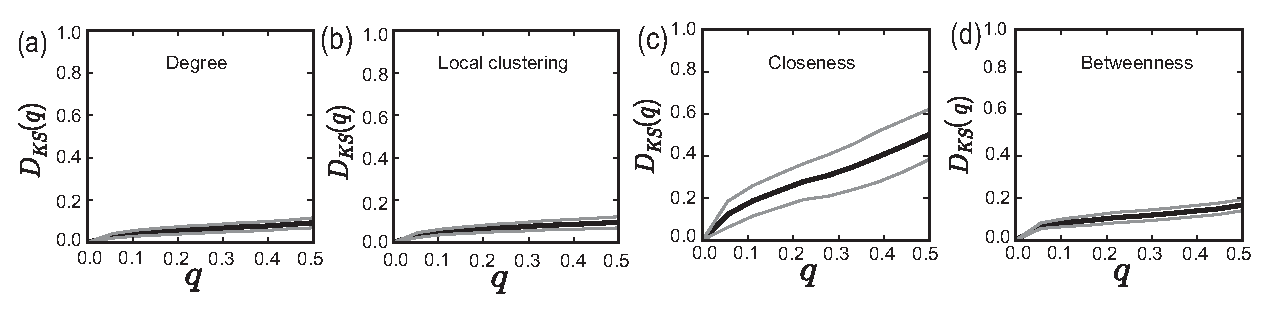
\includegraphics[width=\columnwidth]{Chapter04_VisibilityGt/fig4N.eps}
		  \caption{The Kolmogorov-Smirnov (KS) test statistics $D_{KS}$ versus the fraction $q$ of randomly removed single time series values for the case of a Gaussian white noise time series with $N=100$. (a) Degree $k_i$, (b) local clustering coefficient $\mathcal{C}_i$, (c) closeness $c_i$, and (d) betweenness $b_i$. Missing values are neglected. Black and gray lines correspond to mean values and $\pm 1$ standard deviation levels obtained from $1000$ realizations of the removal process. Modified from \cite{Donner2012}. \label{fig_chap04:missingD}}
		\end{figure}
				
		In real-world applications, missing data often occur not randomly independent of each other, but as blocks. Some further numerical results in this regard can be found in \cite{Donner2012}. 
		
		
		\subsubsection{Homo- and heteroscedastic uncertainties} 
		The influence of measurement uncertainties on the resulting VG properties can be studied in a similar way as for the case of missing values. In particular, Donner {\textit{et al.}} \cite{Donner2012} considered homoscedastic uncertainties as an additional additive Gaussian white noise component, whereas the heteroscedastic case is studied by multiplicative noise with a reasonable, simple analytical distribution. As shown in Fig.~\ref{fig_chap04:homouncertain}, it is found that in both cases the signal-to-noise ratio has a considerable effect by systematically shifting the distributions of vertex properties obtained for the original data towards those expected for the noise process. Note that since in the considered numerical example both signal and noise originated from mutually independent Gaussian white noise processes, there is a saturation of the KS statistics for moderate noise at values corresponding to the variance of VG properties for independent realizations of the same signal process. Further examples of heteroscedastic uncertainties can be found in \cite{Donner2012}. 
		\begin{figure}
		  \centering
		  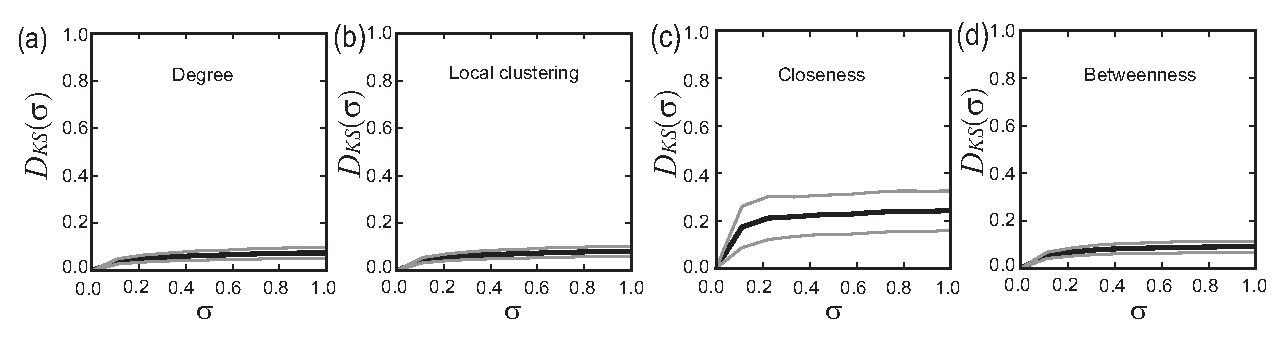
\includegraphics[width=\columnwidth]{Chapter04_VisibilityGt/fig8N.eps}
		  \caption{As in Fig.~\ref{fig_chap04:missingD} for quantifying the effect of additive Gaussian white noise with variance $\sigma^2$ on the VGs for one uncorrelated Gaussian random noise of $N = 100$. Black and gray lines correspond to mean values and $\pm 1$ standard deviation levels obtained from $M=1000$ realizations of the additive noise. Modified from \cite{Donner2012}. \label{fig_chap04:homouncertain}} 
		\end{figure}	
		
		
		\subsubsection{Uneven and irregular timings}
		In a full analogy to the case of uncertainties in the observable $\{x_i \}_{i=1}^N$ with $x_i = x(t_i)$, one can study the impact of uncertain timings $t_i$ on the properties of the resulting VGs. The issue of uncertain timings is a wide-spread problem particularly in the analysis of paleoclimate time series \cite{Telford2004}. Since in the construction of VGs both observable and sampling time enter in terms of an inequality defined by a linear relationship (Eqs.~\ref{vis_cond} and \ref{eq:hvc}), it is not surprising that uncertain timing can indeed have a similar effect on the VG properties as uncertainties in the measurement itself. Figure~\ref{fig_chap04:uncertimings} displays the corresponding KS test statistic results for a realization of Gaussian white noise originally observed with regular spacing, with the timings being corrupted. Note that this specific form of the time-scale corruption, which allows preserving the temporal order of observations, has been inspired by the tent map as a paradigmatic nonlinear mapping often used as an illustrative example in complex systems sciences \cite{Donner2012}. These results demonstrate that the distribution of local vertex properties of a VG are indeed affected by modifications of the time-scale. However, comparing Fig.~\ref{fig_chap04:uncertimings} with Fig.~\ref{fig_chap04:homouncertain}, the changes are considerably smaller than for noisy corruptions of the measurements themselves. The reason for this is that the modification used here has been restricted by the normal sampling interval, whereas the changes induced by additive and multiplicative noise allowed for comparably larger modifications in the data.
		\begin{figure}
		  \centering
		  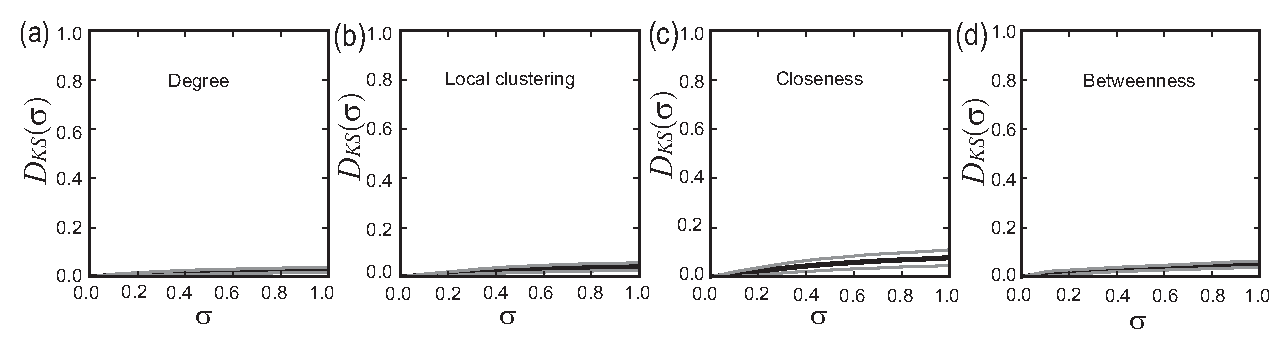
\includegraphics[width=\columnwidth]{Chapter04_VisibilityGt/fig10N.eps}
		  \caption{As in Fig. \ref{fig_chap04:homouncertain} for fixed data, but uncertain timing of observations. Uncertainty in the time domain has been modeled by considering new times $\tilde{t_i} = t_i + \Delta t (| 1 - 2\eta_i | - 0.5)$, where $\eta_i$ are independent realizations of a random variable with uniform distribution in $[0,1]$, and $\Delta t$ is the spacing between subsequent observations in the original data set.  Reproduced from \cite{Donner2012}. \label{fig_chap04:uncertimings}}
		\end{figure}
				
		Uneven timings are paradigmatic for point processes, which are ubiquitous in geoscientific processes, for instance, seismic magnitude series \cite{Telesca2012}. A point process is often characterized by a random time occurrence of the events and these events are typically clustered because they are neither Poissonian nor regularly distributed over time. To check the effects of irregular timing on the degree distributions $p(k)$, Telesca {\textit{et al.}} \cite{Telesca2012} constructed two VGs from (1) the seismic series of the original random occurrence times, and the series (2) that has been substituted by regular conventional time unit. Interestingly, almost identical results have been obtained for $p(k)$, which suggests that the effects of irregular timing are not crucial. However, as we demonstrated in Fig.~\ref{fig_chap04:uncertimings}, network measures are affected by the level of uncertainties in the sampling timings. 

		The trivial connection of neighboring points in time in the (H)VG enhances the signature of structures due to autocorrelations in the record under study. Although this might be desirable for (H)VGs, since some of their respective network properties are explicitly related with the presence of serial dependences (e.g., the typical scale of the degree distribution of HVGs, cf.\, \cite{Luque2009}), there could be situations in which one is interested in removing the corresponding effects. In such cases, it is possible to introduce a minimum time difference for two observations to be connected in the network for removing the effect of slowly decaying auto-dependences, which would correspond to the Theiler window in other concepts of nonlinear time series analysis \cite{Theiler1986}.
		
		We note that other than for VGs or related methods, the uncertain timings or irregular time spacings can have substantial effects on the construction of ordinal pattern transition networks \cite{Kulp2016a,McCullough2016,Sakellariou2016}, which will be reviewed in Section \ref{sec:TransitionNt}. Furthermore, the current discussion is limited to the case of a Gaussian white noise process and more generalizations to non-Gaussian assumptions are necessary to be explored, which are much closer to the situations of real time series. 


	\subsection{Multivariate visibility graph methods}
	Despite their success, the range of applicability of (H)VGs methods has been mainly limited to univariate time series, although the most challenging problems in the area of nonlinear science concern systems that are described by multivariate time series. Synchronization analysis is one of traditional topics when generalizing (H)VG analysis from a univariate to bivariate time series \cite{Ahmadlou2012a,Mitra2012}. We notice that there are several different ways of extending the ideas from a single time series to multivariate time series, for instance, multiplex VGs, cross-VGs and joint VGs. For instance, the cross-visibility algorithm has been proposed to understand coupling and information transfer between two time series \cite{Mehraban2013}. Here, we summarize some of the different approaches to characterize bivariate time series using (H)VGs. 
	
		\subsubsection{Multiplex visibility graphs} \label{sec:multiplexVG}
		Based on the definition of HVGs, Lacasa \textit{el al.} \cite{Lacasa2015b} proposed to transform a multidimensional time series into an appropriately defined multiplex visibility graph. New information can be extracted from the original multivariate time series, with the aims of describing signals in graph-theoretical terms or to construct novel feature vectors to feed automatic classifiers in a simple, accurate and computationally efficient way. Multiplex VG analysis has been applied to characterize the heterogeneity of recurrent neural network dynamics \cite{Bianchi2017} and different conditions of resting state human fMRI data \cite{Sannino2017}. 
		
		Consider an $M$-dimensional real valued time series $\{ \vec{x}_i \} = (\{ x_i^{[1]}\}, \{x_i^{[2]} \}, \dots, \{x_i^{[M]} \})$ with $\vec{x}_i = \vec{x}(t_i)  \in \mathbb{R}^M$ for any value of $t_i \in [1, N]$, measured empirically or extracted from an $M$-dimensional, either stochastic or deterministic dynamical system. In full analogy to the notation used for describing multiplex recurrence networks in Section~\ref{sec:mrn}, the superscript index represents here the $\alpha$-th variable. An $M$-layer multiplex visibility graph $\mathcal{M}$ is then constructed, where layer $\alpha$ corresponds to the HVG associated to the time series $\{ x_i^{[\alpha]}\}_{t_i=1}^{N}$ of state variable $X^{[\alpha]}$. Note that $\mathcal{M}$ is represented by the vector of adjacency matrices of its layers $\mathbf{\mathcal{A}} = \{\mathbf{A}^{[1]}, \mathbf{A}^{[2]}, \dots, \mathbf{A}^{[M]}\}$, where $\mathbf{A}^{[\alpha]} = \{A_{ij}^{[\alpha]} \}_{ij}$ is the adjacency matrix of layer $\alpha$. Such a mapping builds a bridge between multivariate series analysis and recent developments in the theory of multilayer networks \cite{Boccaletti2014}, making it possible to employ the structural descriptors introduced to study multiplex networks as a toolbox for the characterization of multivariate signals. 
		
		Two measures have been proposed to capture, respectively, the abundance of single edges across layers and the presence of inter-layer correlations of node degrees \cite{Lacasa2015b}, which help to characterize information shared across variables (layers) of the underlying high dimensional system. Simply speaking, we compute the two measures defined by Eqs.~(\ref{eq:RNmultiplex},\ref{eq:RNmultiplexW}), which are based on the adjacency matrices of HVGs. More specifically, the first measure is the \textit{average edge overlap} $\omega$ (Eq.~\ref{eq:RNmultiplexW}),  	
%		The first measure is the average edge overlap
%\begin{equation} \label{eq:VGmultiplexW}
%\omega = \frac{\sum_i\sum_{j>i} \sum_{\alpha}a_{ij}^{[\alpha]}}{M \sum_i\sum_{j>i}(1-\delta_{0, \sum_{\alpha}a_{ij}^{[\alpha]}})}
%\end{equation}
which computes the expected number of layers of the multiplex on which an edge is present. Note that $\omega$ takes values in $[1/M, 1]$ and in particular $\omega = 1/M$ if each edge $(i,j)$ exists in exactly one layer, i.e. if there exist a layer $\alpha$ such that $A_{ij}^{[\alpha]} = 1$ and $A_{ij}^{[\beta]} = 0$\, $\forall\, \beta \neq \alpha$, while $\omega = 1$ only if all the $M$ layers are identical. As a consequence, the average edge overlap of a multiplex VG can be used as a proxy of the overall coherence of the original multivariate time series, with higher values of $\omega$ indicating high correlation in the microscopic structure of the signal. 

		The second measure proposed in \cite{Lacasa2015b} allows to quantify the presence of \textit{interlayer correlation} between the degrees of the same node at two different layers. More specifically, given a pair of layers $\alpha$ and $\beta$ of $\mathcal{M}$, respectively characterized by the degree distributions $p(k^{[\alpha]})$ and $p(k^{[\beta]})$, the interlayer correlation is defined by the mutual information $I^{\alpha\beta}$ (Eq.~\ref{eq:RNmultiplex}) between $p(k^{[\alpha]})$ and $p(k^{[\beta]})$. % as 
%		\begin{equation} \label{eq:VGmultiplex}
%		I_{\alpha, \beta} = \sum_{k^{[\alpha]}} \sum_{k^{[\beta]}} P(k^{[\alpha]}, k^{[\beta]}) \log \frac{P(k^{[\alpha]}, k^{[\beta]})}{P(k^{[\alpha]}) P(k^{[\beta]}) }, 
%		\end{equation}
		% where $p(k^{[\alpha]}, k^{[\beta]}) $ is the joint probability to find a node having degree $k^{[\alpha]}$ at layer $\alpha$ and degree $k^{[\beta]}$ at layer $\beta$. 
		The higher $I^{\alpha\beta}$ the more correlated are the two layers and therefore the structures of the associated time series. Then, the average of $I^{\alpha \beta}$ over every pair of layers of $\mathcal{M}$ gives a scalar variable $I = \left < I^{\alpha\beta}\right>_{\alpha, \beta}$, which captures the amount of information flow in the multivariate time series. 
		
		Note that the interlayer correlation gives a weighted correlation matrix of size $M \times M$ and each entry is represented by $I^{\alpha\beta}$. That means that the original $M$-dimensional time series is transformed to a weighted graph of $M$ nodes, where each node represents one layer and the weights of the edges denote the magnitude of mutual information computed from the associated (H)VG degree distributions.  
        
        
		\subsubsection{Joint and excess degrees} \label{subsec:jointdegreeVG}
		Some network-theoretic quantities to quantify asymmetries in bivariate time series have been introduced in \cite{Zou2014}. Following the notations as described for multiplex (H)VG, we restrict here our considerations to two-dimensional time series which results in two layers $\alpha$ and $\beta$. For $\{x^{[\alpha]}_i\}_{i=1}^{N}$ and $\{x^{[\beta]}_i\}_{i=1}^{N}$, we again consider two (H)VGs with adjacency matrices $\mathbf{A}^{[\alpha]}$ and $\mathbf{A}^{[\beta]}$, respectively. Note that the sets of vertices are the same for both subgraphs, with differences exclusively in the set of edges.

Based on the thus obtained (H)VGs, we proceed as follows:
\begin{enumerate}
\item From the two (H)VGs, we have two sets of neighbors, $\mathcal{N}_i^{[\alpha],[\beta]} = \left\{ A_{ij}^{{[\alpha]}, {[\beta]}} \equiv 1, j \in \left\{1,\ldots, N \right\}/\left\{i\right\} \right\}$ for each time $i \in \left\{1,\ldots, N \right\}$. The \textit{degree sequences} are then defined as
\begin{align}
&k_i^{{[\alpha]}, {[\beta]}} = \# \mathcal{N}_i^{{[\alpha]}, {[\beta]}} = \sum_{j} A_{ij}^{{[\alpha]}, {[\beta]}}.
\end{align}

\item The \textit{joint degree}
\begin{align} \label{eq:jointK}
&k_i^\textrm{joint} = \# \left( \mathcal{N}_i^{{[\alpha]}} \cap \mathcal{N}_i^{{[\beta]}} \right) = \sum_{j} A_{ij}^{{[\alpha]}}\cdot A_{ij}^{{[\beta]}}
\end{align}
gives the number of common neighbors of a vertex corresponding to time $i$ in both sequences. Notably, we can define $\{k_i^{joint}\}$ as the degree sequence of a \textit{joint} (H)VG combining the visibility criteria for two distinct time series. Here, the adjacency matrix is defined by the point-wise multiplication of the individual (H)VGs' adjacency matrices. This idea is conceptually related to the concept of joint recurrence plots encoding the simultaneous recurrence of two dynamical systems in their respective phase spaces \cite{romano2004}. One simple idea is to compare the cross correlation or mutual information between the two degree sequences of $\{k_i^{[\alpha]}\}$ and $\{k_i^{[\beta]}\}$ \cite{Lacasa2015b,Ahmadi2018}. 

\item In a similar spirit as the joint degree sequence, we can quantify the number of edges associated with time $i$, which connect to vertices contained in $\mathcal{N}_i^{{[\alpha]}}$ but \textit{not} in $\mathcal{N}_i^{{[\beta]}}$, or vice versa. More specifically,
\begin{align}
k_i^{{o,[\alpha]}} & = \# \left( \mathcal{N}_i^{{[\alpha]}} \cap \overline{\mathcal{N}_i^{{[\beta]}}} \right)  =  \sum_{j} A_{ij}^{{[\alpha]}}\cdot \left( 1-A_{ij}^{{[\beta]}} \right) \\
k_i^{{o,[\beta]}} & = \# \left( \mathcal{N}_i^{{[\beta]}} \cap \overline{\mathcal{N}_i^{{[\alpha]}}} \right) = \sum_{j} A_{ij}^{{[\beta]}}(t)\cdot \left(1-A_{ij}^{{[\alpha]}} \right)
\end{align}
where $\overline{\mathcal{N}_i^{{[\alpha]}, {[\beta]}}(t)}=\{1,\ldots,T\}\cap \left\{ \mathcal{N}_i^{{[\alpha]}, {[\beta]}}\cup i\right\}$ is the complementary set of $\mathcal{N}_i^{{[\alpha]}, {[\beta]}}$, which measures the number of neighbors that belong \textit{only} to $\mathcal{N}_i^{{[\alpha]}}$ or $\mathcal{N}_i^{{[\beta]}}$, respectively. Therefore, we refer $k_i^{o,{[\alpha]}, {[\beta]}}$ as the \textit{conditional degree sequences}. By definition,
\begin{align}\label{eq:nad}
k_i^{o,{[\alpha]}, {[\beta]}}=k_i^{{[\alpha]}, {[\beta]}}-k_i^\textrm{joint}.
\end{align}
\end{enumerate}

Based on the latter definitions (Eq.~\ref{eq:nad}), we compute the following properties:
\begin{align} \label{eq:deltaK}
\Delta k_i &= k_i^{o,{[\alpha]}} - k_i^{o,{[\beta]}} = k_i^{{[\alpha]}} - k_i^{{[\beta]}} \\ \label{eq:deltaReK}
\Delta_{rel} k_i &= \Delta k_i/\left(k_i^{{[\alpha]}} + k_i^{{[\beta]}} \right).
\end{align}
The \textit{excess degree} $\Delta k_i$ quantifies how much ``more convex'' the fluctuations of $\mathbf{A}^{[\alpha]}$ are in comparison with $\mathbf{A}^{[\beta]}$ around a given time $i$ (i.e., how many more or less visibility connections the observation of $\mathbf{A}^{[\alpha]}$ at time $i$ obeys in comparison with $\mathbf{A}^{[\beta]}$). By additionally considering the \textit{relative excess degree} $\Delta_{rel} k_i$ normalized by the sum of the individual degrees, we obtain a measure that does not exhibit marked sensitivity with respect to the actual degrees $k_i^{{[\alpha]}, {[\beta]}}$, which may considerably vary over time according to the statistical and dynamical characteristics of the data.

In Section~\ref{subsec:sunspotsAsym}, we will summarize the applications of $\Delta k_i$ and $\Delta_{rel} k_i$ to characterize the north--south asymmetry of solar activity \cite{Zou2014}, which provide many nonlinear properties that have not been studied by other methods. Notably, this approach is conceptually related with recently developed (H)VG-based tests for time series irreversibility, which compare (among others) degree distributions obtained when considering edges to past and future observations separately \citep{Donges2013}. We will address these methods in the following.

        \subsubsection{Visibility graph similarity}
						
As an early alternative to studying inter-layer similarities in multiplex (H)VGs, Ahmadlou and Adeli \cite{Ahmadlou2012a} introduced the concept of visibility graph similarity. Here, a combination of ideas from time delay embedding, recurrence analysis and visibility graphs is used to quantify the statistical relationship between two observed sequences. For this purpose, each sequence is first subjected to classical time delay embedding. Next, a certain state vector from the previously constructed set is chosen as a reference, and a time series of distances with respect to this reference point is constructed. For the resulting time series of distances, the corresponding VG is constructed. Finally, by pair-wise comparison between the thus obtained VG degree sequences obtained for the two time series of interest in terms of their correlation coefficient, a VG-based similarity measure is constructed, which has been used for capturing signatures of generalited synchronization in paradigmatic model systems \cite{Ahmadlou2012a}, but also for constructing time-dependent functional network representations of human brain actvity from multi-channel EEG measurements \cite{Sengupta2013}.

                        
	\subsection{Decomposition of visibility graphs} \label{sec:timeIRvg}
		\subsubsection{Time-directed visibility graphs and characterizations}
		So far, visibility graphs have mostly been considered as undirected, since visibility does not have a predefined temporal arrow. However, (H)VGs be made directed by again assigning to the links a time arrow, which result in the so called directed VGs and HVGs. Accordingly, a link between $i$ and $j$ (where time ordering yields $i< j$) generates an outgoing link for $i$ and an incoming link for $j$. Therefore, the degree $k_i$ of the node $i$ is now split into an in-degree $k_i^{in}$, and an out-degree $k_i^{out}$, such that $k_i= k_i^{in}+k_i^{out}$. The in-degree $k_i^{in}$ is defined as the number of links of node $i$ with other past nodes associated with data in the series (that is, nodes with $j < i$). Conversely, the out-degree $k_i^{out}$, is defined as the number of links with future nodes. Then we define the in- and out-degree distributions of a directed VG (HVG) as $p(k^{out})$ and $p(k^{in})$, respectively. An important property at this point is that the ingoing and outgoing degree sequences are interchangeable under time reversal. 
		
		More specifically, given the adjacency matrix $\mathbf{A}$ of a (H)VG, the degree {$k_i =\sum_{j} A_{ij}$} measures the number of edges incident to a given vertex {$i$}. Then, Donges \textit{et~al.} \cite{Donner2012Nolta,Donges2013} adapted a somewhat different yet equivalent notation for in- and out-degree sequences. More specifically, they decomposed the quantity $k_i$ for a vertex corresponding to a measurement at time $i$ into contributions due to other vertices in the past and future of $i$,
\begin{eqnarray} \label{eq:kvin}
k_i^r &= \sum_{j<i} A_{ij},\\ \label{eq:kvout}
k_i^a &= \sum_{j>i} A_{ij}
\end{eqnarray}
with $k_i=k_i^r+k_i^a$, being referred to as the \emph{retarded} and \emph{advanced degrees}, respectively. Here, $k_i^r$ and $k_i^a$ correspond to the respective in- and out-degrees of time-directed (H)VGs \cite{Lacasa2012}. While the degrees of an individual vertex can be significantly biased due to the finite time series length~\cite{Donner2012}, the resulting frequency distributions of retarded and advanced degrees are equally affected. 

		The local clustering coefficient $\mathcal{C}_i = {k_i \choose 2}^{-1} \sum_{j,k} A_{ij} A_{jk} A_{ki}$ is another vertex property of higher order characterising the neighbourhood structure of vertex $i$~\cite{Newman2003}. Here, for studying the connectivity due to past and future observations separately, \cite{Donges2013} defined the \emph{retarded} and \emph{{advanced local clustering coefficients}}
\begin{eqnarray} \label{eq:cvin}
\mathcal{C}_i^r &= {k_i^r \choose 2}^{-1} \sum_{{j<i,k<i}} A_{ij} A_{jk} A_{ki},\\ \label{eq:cvout}
\mathcal{C}_i^a &= {k_i^a \choose 2}^{-1} \sum_{{j>i,k>i}} A_{ij} A_{jk} A_{ki}.
\end{eqnarray}
Hence, both quantities measure the probability that two neighbours in the past (future) of observation $i$ are mutually visible themselves. Note that the decomposition of $\mathcal{C}_i$ into retarded and advanced contributions is not as simple as for the degree and involves degree-related weight factors and an additional term combining contributions from the past and future of a given vertex.

		Finally, {we note that} other measures characterising complex networks on the local (vertex/edge) as well as global scale could be used for similar purposes as {those} studied in this work. However, {since} path-based network characteristics {(e.g.,} closeness, betweenness, or average path length{)} cannot be easily decomposed into retarded and advanced contributions, the approach followed here is mainly restricted to neighbourhood-based network measures like degree, local and global clustering coefficient, or network transitivity. As a possible solution, instead of decomposing the network properties, the whole edge set of a (H)VG could be divided into two disjoint subsets that correspond to visibility connections forward and backward in time, as originally proposed by Lacasa~\textit{et~al.}~\cite{Lacasa2012}. For these directed (forward and backward) (H)VGs, also the path-based measures can be computed separately and might provide valuable information. 
		
		\subsubsection{Tests for time series irreversibility}
		Testing for nonlinearity of time series has been of great interest. Various approaches have been developed for identifying signatures of different types of nonlinearity as a necessary precondition for the possible emergence of chaos. Since linearity of Gaussian processes directly implies time-reversibility \cite{Weiss1975,Lawrance1991,Diks1995}, nonlinearity results (among other features) in an asymmetry of certain statistical properties under time-reversal~\cite{Theiler1992}. Therefore, studying reversibility properties of time series is an important alternative to the direct quantitative assessment of nonlinearity~\cite{Voss1998}. In contrast to classical higher-order statistics requiring surrogate data techniques~\cite{Theiler1992}, most recently developed approaches for testing irreversibility have been based on symbolic dynamics~\cite{Daw2000,Kennel2004,Cammarota2007} or statistical mechanics concepts~\cite{Costa2005,Porporato2007,Roldan2010}. 
		
		The time series reversibility has the following definition: a time series $\Sigma = \{ x_1, x_2, \dots, x_n \}$ is called statistically time reversible if the time series $\Sigma^{\ast} = \{x_{-1}, x_{-2}, \dots, x_{-n} \}$ has the same joint distribution as $\Sigma$. Therefore, time reversibility implies stationarity \cite{Lawrance1991}. By this definition, time series reversibility reduces to the equivalence between forward and backward statistics and hence, nonstationary series are infinitely irreversible and therefore $\Sigma$ and $\Sigma^{\ast}$ have different statistics that increase over time \cite{Weiss1975}. More specifically \cite{Lawrance1991}, time-{ir}reversibility of a stationary stochastic process or time series $\{x_i\}$ requires that for arbitrary $n$ and $m$, the tuples $(x_n,x_{n+1},\dots,x_{n+m})$ and $(x_{n+m},x_{n+m-1},\dots,x_n)$ have the same joint probability distribution. It is practically unfeasible in most situations due to the necessity of estimating high-dimensional probability distribution functions from a limited amount of data. Instead of testing this condition explicitly, for detecting time series irreversibility it can be sufficient to compare the distributions of certain statistical characteristics obtained from both vectors (e.g.,~\cite{Tong1990}). In the following, we will review the corresponding VG-based approaches.

		\paragraph{Kullback-Leibler divergence}
		In many applications, one can actually quantify different kinds of time asymmetries in the underlying dynamics on nonstationary processes. Following previous work \cite{Lacasa2012}, the topological properties of (H)VGs associated to several types of nonstationary processes have been proposed to quantify different degrees of irreversibility of several nonstationary processes \cite{Lacasa2015}. Furthermore, they take advantage of the fact that the topological properties of these graphs are effectively invariant under time shift for large classes of nonstationary processes, which allows to introduce the concept of visibility graph stationarity. This in turn allows to extract meaningful information on the time asymmetry of nonstationary processes. 

		Lacasa \textit{et al.} \cite{Lacasa2015} defined time series reversibility in terms of (H)VGs in the following way: a time series $\Sigma = \{ x_i \}_{i=1}^N$ is said to be (order $p$) (H)VG reversible if and only if, for large $N$, the order $p$ block ingoing and outgoing degree distribution estimates of the directed (H)VG associated to $\Sigma$ are asymptotically identical, i.e., 
\begin{equation}
p(k_1^{in}, k_2^{in}, \dots, k_p^{in}) = p(k_1^{out}, k_2^{out}, \dots k_p^{out}).
\end{equation}
This property yields that the ingoing and outgoing degree sequences of the original and time reversed series have the same distribution, namely, 
\begin{equation}
p(k^{in}) [\Sigma] = p(k^{out}) [ \Sigma^{\ast}]; p(k^{out}) [\Sigma] = p(k^{in})[\Sigma^{\ast}],  
\end{equation}
where $\Sigma^{\ast} = \{ x_{n+1-i} \}_{i=1}^{n}$ represents the time reversed series. For time series, we assess how close the system is to reversibility by quantifying the distance between $p(k^{in})$ and $p(k^{out})$.  

		The distance between the \textit{in} and \textit{out} degree distributions has been calculated by the Kullback-Leibler divergence (KLD) \cite{Lacasa2012,Lacasa2015}, which is used in information theory as a measure to distinguish between two probability distributions. More specifically, the KLD between these two distributions is
\begin{equation}\label{eq:KLD}
D_{k l d}(in \| out) = \sum_{k} p(k^{in}) \log \frac{p(k^{in})}{p(k^{out})}. 
\end{equation}
This measure $D_{k l d}(in\|out)$ is a semi-distance which vanishes if and only if the outgoing and ingoing degree probability distributions of a time series are identical, but is positive otherwise. Then the (H)VG reversibility is redefined if the following expression holds:
\begin{equation}
\lim_{N \to \infty} {D_{k l d}(in\|out)} = 0. 
\end{equation}		
Truly irreversible process have positive values of Eq.~\eqref{eq:KLD} in the limit of large $N$ \cite{Lacasa2012}. The consistency of this test for HVGs has been demonstrated numerically for chaotic dissipative systems (HVG-irreversible), long-range dependent stochastic processes (HVG-reversible) \cite{Lacasa2012} and non-Markovian random walks (HVG-irreversible) \cite{Lacasa2015}.

		Lacasa \textit{et al.}\cite{Lacasa2012, Lacasa2015} conjectured that the information stored in the in- and out-degree distributions takes into account the amount of time irreversibility of the associated series. More precisely, they suggested that this can be measured, in a first approximation, as the distance (in a distributional sense) between the in- and out-degree distributions ($p(k^{in})$ and $p(k^{out})$). This claim was recently supported by quantitative numerical analysis of $D_{k l d}$ for a modified Langevin equation and some simple population growth model with tunable long-range dependence \cite{Telesca2018c}. Specifically, it was found that both persistence and anti-persistence increase the value of the Kullback-Leibler divergence, with the effect of positive correlations being somewhat stronger than that of negative ones.
        
        Instead of degree based characteristics, higher order measures can be used as well if necessary, such as the corresponding distance between the in and out degree-degree distributions ($p(k^{in}, k'^{in})$ and $p(k^{out}, k'^{out})$). These are defined as the in and out joint degree distributions of a node and its first neighbors, describing the probability of an arbitrary node whose neighbor has degree $k'$ to have degree $k$. That is, we compare the out-degree distribution in the actual (forward) series $p(k^{out})$ with the corresponding probability in the time-reversed (or backward) time series, which is equal to the probability distribution of the ingoing degree in the actual process. 
		
		Therefore, by calculating Eq.~\eqref{eq:KLD}, Lacasa \textit{et al.}\cite{Lacasa2012} have shown that one can correctly distinguish between reversible and irreversible stationary time series, including analytical and numerical studies of its performance for: (i) reversible stochastic processes (uncorrelated and Gaussian linearly correlated), (ii) irreversible stochastic processes, (iii) reversible (conservative) and irreversible (dissipative) chaotic maps, and (iv) dissipative chaotic maps in the presence of noise. Numerical examples of time irreversibility tests have been provided in Fig.~\ref{fig:chapter4timeReverse}. In particular, they first considered time series of length $2^{15}$ from white noise of $i.i.d.$ uniformly random uncorrelated variables $\sim U[0,1]$ (Fig. \ref{fig:chapter4timeReverse}(a,b)). In this case, Fig.~\ref{fig:chapter4timeReverse}(a) shows that both distributions are identical up to finite-size effects fluctuations. In addition, the irreversibility measure $D_{k l d}(in\|out)$ vanishes asymptotically as $1/N$, showing that finite irreversibility values for finite size are due to statistical fluctuations that vanish asymptotically. Therefore, Fig.~\ref{fig:chapter4timeReverse}(a, b) suggest that the underlying process is time reversible. In contrast, both distributions are clearly different for the chaotic logistic map (Fig.~\ref{fig:chapter4timeReverse}(c)), which is further confirmed by the convergence of $D_{k l d}(in\|out)$ to a finite value with $N$ (Fig.~\ref{fig:chapter4timeReverse}(d)). Therefore, the logistic map is time irreversible. 
		\begin{figure}[htbp]
		\centering
			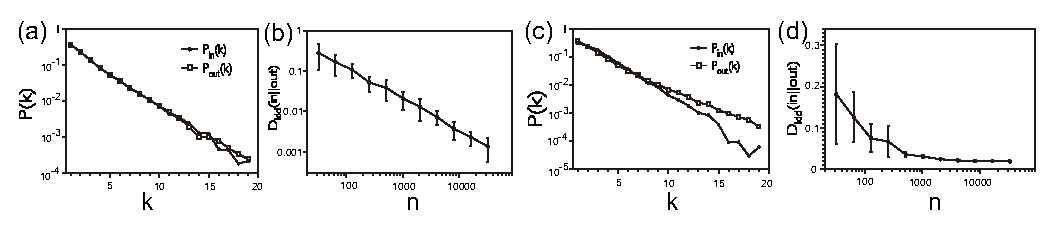
\includegraphics[width=\columnwidth]{Chapter04_VisibilityGt/timeReverse.eps}
			\caption{Time irreversibility testing for white noise (a,b) and the chaotic logistic map (c,d). (a,c) Semi-logarithmic plots of the in- and out-degree distributions of the VG. (b,d) Time irreversibility measure $D_{k l d}(in\|out)$ versus series size $N$. Modified from \cite{Lacasa2015} with permission by American Physical Society. } \label{fig:chapter4timeReverse}
		\end{figure}
		
		Notice that the majority of previous methods to estimate time series irreversibility generally proceed by first making a (somewhat ad hoc) local symbolization of the series, coarse-graining each of the series data into a symbol (typically, an integer) from an ordered set ~\cite{Daw2000,Kennel2004,Cammarota2007,Costa2005,Porporato2007,Roldan2010}. The method based on directed (H)VGs here lacks an ad hoc symbolization process, which may in principle take into account multiple scales. The unnecessary requirement of symbolization is desirable if we want to tackle complex signals and, hence, it can be applied directly to any kind of real-valued time series.  

		We note that (H)VG reversibility varies depending on the detailed properties of particular processes \cite{Lacasa2015,Telesca2018c}, which calls for careful interpretations. For instance, both analytical calculations and numerical simulations show that unbiased additive random walks, while nonstationary, are both (H)VG  stationary and (H)VG time reversible. On the other hand, biased memoryless additive random walks are HVG irreversible with finite irreversibility measures that quantify the degree of time asymmetry, while these are still VG reversible, as VGs are invariant under superposition of linear trends in the original data. Numerical examples suggest that HVGs can capture, for both finite and infinite series size, the irreversible nature of non-Markovian additive random walks, whereas VGs are only able to do so for finite series. For multiplicative random walks, the processes are HVG reversible if the process is akin to an unbiased additive process in logarithmic space, and time irreversible if the process reduces to a biased additive process in logarithmic space. Finally, the VGs capture the time irreversible character of multiplicative random walks, yielding finite values in the unbiased case and asymptotically diverging quantities in the biased case. Furthermore, these conclusions are based on the limit of infinitely long time series $N \to \infty$ and finite size time series always yield finite, non-zero values of HVG and VG irreversibility \cite{Xiong2018}, which needs a proper test justifying the statistical significance. 
		
		\paragraph{Kolmogorov-Smirnov (KS) test for irreversibility}
		While the results of the KLD measure for reversible and irreversible dynamics quantitatively differ in several orders of magnitude, a statistical test is required. Lacasa \textit{et al.} \cite{Lacasa2012} proposed to address the statistical significance by surrogate techniques as follows: one first proceeds to shuffle the series under study in order to generate a randomized resampled data set with the same underlying probability density. This resampled series, whose irreversibility measure is asymptotically zero, is considered as the null hypothesis of the test. Recently, a combination of Kullback-Leibler distance between the ingoing and outgoing degree sequences and the so-called inversion number of the permutation of the original time series has been proposed to characterize asynchronous patterns of time irreversibility \cite{Yang2018}. Taking a slightly different algorithm, Donges \textit{et~al.} \cite{Donner2012Nolta,Donges2013} have extended this idea and proposed to utilize some standard statistics for testing the homogeneity of the distribution of random variables between two independent samples, which can be formulated for both standard and horizontal VGs and for different network properties. 
		
		More specifically, following the decomposition of vertex properties into time-directed contributions proposed above (including network degrees and local clustering coefficients, Eqs.~(\ref{eq:kvin})-(\ref{eq:cvout})), Donges {\textit{et al.}} \cite{Donges2013} utilized the frequency distributions {$p(k^{r})$ and $p(k^{a})$ ($p(\mathcal{C}^{r})$ and $p(\mathcal{C}^{a})$)} of retarded and advanced {vertex properties} as representatives for the statistical properties of the time series when viewed forward and backward in time. In the case of time-reversibility, they conjecture that both sequences {$\{k_i^{r}\}$ and $\{k_i^{a}\}$} (or {$\{\mathcal{C}_i^{r}\}$ and $\{\mathcal{C}_i^{a}\}$}) should be drawn from the same probability distribution, because the visibility structure towards the past and future of each observation has to be statistically equivalent. In turn, for an irreversible (i.e., nonlinear) process, we expect to find statistically significant deviations between the probability distributions of retarded and advanced characteristics. In other words, rejecting the null hypothesis that {$\{k_i^{r}\}$ and $\{k_i^{a}\}$} ({$\{\mathcal{C}_i^{r}\}$ and $\{\mathcal{C}_i^{a}\}$}) are drawn from the same probability distribution, respectively, implies rejecting the null hypothesis that the time series under investigation is reversible. 
		
		{Since for sufficiently long time series (representing the typical dynamics of the system under study), the available samples of individual vertex properties approximate the underlying distributions sufficiently well, we can (despite existing correlations between subsequent values)} consider the Kolmogorov-Smirnov (KS) test for testing this null hypothesis. {Specifically}, a small $p$-value of the KS test statistic (e.g., $p<0.05$) implies that the time series has likely been generated by an irreversible stochastic process or dynamical system. Even more, these $p$-values are distribution-free in the limit of $N\to\infty$. {Neglecting possible effects of the intrinsic correlations between the properties of subsequent vertices on the estimated $p$-values (which shall be addressed in future research), this} implies that we do \textit{not} need to construct surrogate time series for obtaining critical values of our test statistics as in other {ir}reversibility tests. Note that other (not network-related) statistical properties sensitive to the time-ordering of observations could also be exploited for constructing similar statistical tests for time series irreversibility \cite{Donges2013}. 
		
		The KS test for irreversibility has been demonstrated by model time series of AR(1) process ($p = 1, \varphi_1 = 0.5$ in Eq.~\eqref{def:AR}) and the chaotic H\'enon map (Eq.~\eqref{eq:henon}) as shown in Fig. \ref{fig:chapter4KSReverse}. For the linear (reversible) AR(1) process, the empirical distributions of retarded/advanced {vertex properties} collapse onto each other \cite{Donges2013}. Consequently, the null hypothesis of reversibility is never rejected by the test based on the degree (Fig.~\ref{fig:chapter4KSReverse}(a)), and only rarely rejected by the clustering-based test well below the expected false rejection rate of 5\% (Fig.~\ref{fig:chapter4KSReverse}(b)). In contrast, for the irreversible H\'enon map, the null hypothesis of reversibility is nearly always (degree, Fig.~\ref{fig:chapter4KSReverse}(c)) or always (local clustering coefficient, Fig.~\ref{fig:chapter4KSReverse}(d)) rejected. To further evaluate the performance of the tests for varying series size $N$, the receiver operating characteristics (ROC curves) have been applied to quantify the false positive rate versus true positive rate when testing irreversibility \cite{Donges2013}. 		
		\begin{figure}[htbp]
		\centering
			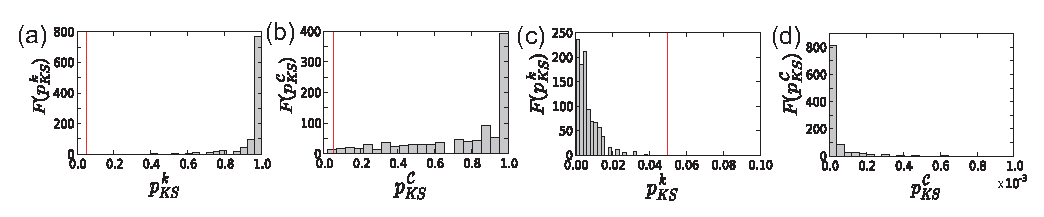
\includegraphics[width=\columnwidth]{Chapter04_VisibilityGt/ks_reverse.eps}
			\caption{(color online) Frequency distributions of $p$-values of the KS statistic for comparing the distributions of retarded/advanced (a,c) degree {$k_i^{r}$, $k_i^{a}$} and (b,d) local clustering coefficient {$\mathcal{C}^{r}_i$, $\mathcal{C}^{a}_i$} of standard VGs from an ensemble of $M=1,000$ realizations of model system time series of length $N=500$: (a,b) AR(1) process, (c,d) H\'enon map. Vertical red lines indicate the typical significance level of 0.05 {where appropriate (note the different scale in panel (d))}.  Modified from \cite{Donges2013}. } \label{fig:chapter4KSReverse}
		\end{figure}

		Utilizing standard as well as horizontal VGs for discriminating between the properties of observed data forward and backward in time has at least two important benefits: (i) {Unlike for some classical tests (e.g.,~\cite{Theiler1992}),} the reversibility properties are examined without the necessity of constructing surrogate data. Hence, the proposed approach saves considerable computational costs in comparison with {such methods} and, more importantly, avoids the problem of selecting a particular type of surrogates. Specifically, utilizing the KS test statistic or a comparable two-sample test for the homogeneity (equality) of the underlying probability distribution functions directly supplies a $p$-value for the associated null hypothesis that the considered properties of the data forward and backward in time are statistically indistinguishable. (ii) The proposed approach {is applicable} to data with non-uniform sampling {(common in areas like} paleoclimate~\cite{Donner2012,Donner2012Nolta} or astrophysics) {and} marked point processes (e.g., earthquake catalogues~\cite{Telesca2012}). For {such} data, constructing surrogates for {non}linearity tests in the most common way {using} Fourier-based techniques is a challenging task, {which is avoided by} {(H)}VG-based methods. 

		We emphasize that this method exploits the time-information explicitly used in constructing (H)VGs. Other existing time series network methods (e.g., recurrence networks \cite{Marwan2009,Donner2010a,Donner2011}) not exhibiting this feature cannot be used for the same purpose. Furthermore, there are methodological questions such as the impacts of sampling, observational noise, and intrinsic correlations in vertex characteristics as well as a detailed comparison to existing methods for testing time series {ir}reversibility that need to be systematically addressed in future research. Furthermore, {(H)}VG-based methods are generally faced with problems such as boundary effects and the ambiguous treatment of missing data \cite{Donner2012}, which call for further investigations, too. 
		
		It may be noted that unlike neighborhood-based network measures like degree and local clustering coefficients, path-based measures of (H)VGs are known to be strongly influenced by boundary effects \cite{Donner2012}, so that they could possibly lose their discriminative power if employed in a similar fashion in the context of {ir}reversibility tests. 
        
        Irreversibility tests have been conducted for various real valued time series. Examples include neuro-physiological EEG recordings \cite{Donges2013}, mean temperature anomaly series \cite{Xie2014}, financial time series \cite{Flanagan2016}, oil-water two-phase flows \cite{Meng2016a}, meteorological stream flow fluctuations \cite{Serinaldi2016}, correlated fractal processes \cite{Xiong2018}, and seismic sequences of a Mexican subduction zone \cite{Telesca2018}. 
		
		
		
		
		
		
